\documentclass[main.tex]{subfiles}
\begin{document}
\pagestyle{empty}

\newgeometry{a4paper,left=1in,right=1in,top=1in,bottom=1in,nohead}

%%%%%%%%%%%%HEADING TITLE
\hfill
\vspace{0.2cm}
\begin{center}
{\large \bfseries 
EXPERIMENT 
\par
\Huge
Molecular geometry
\\[5pt] \par}
\vspace{0.2cm}
\end{center}
\par

%\uline{  \hfill \normalsize \hfill       }
%%%%%%%%%%%%HEADING
\vspace{0.2cm}{\large \bfseries Goal}
This experiment will go over the ideas of molecular geometry and bond-hybridization. On one hand, you will learn how to predict the geometry of a molecule and how to differentiate, for example, a linear molecule from a bent molecule. Also you will learn to predict the hybridization of atomic orbitals involved in a chemical bond.


\vspace{0.2cm}{\large \bfseries Background}
Molecules result from the combination of atoms. For example, a \ce{H2O} molecule results of the combination of one oxygen atom with two hydrogen atoms. The atoms of a molecule combine by exchanging or sharing electrons, depending on the type of bond. Water is a covalent molecule and the oxygen and hydrogen atoms share the electrons in the bond. Only electrons in the outermost electron shell participate in chemical bonds. Those electrons are called \text{valence electrons}. Core electrons, electrons in inner shells of the atom, do not participate in chemical bonds. The electron configuration of oxygen is $1s^2$\textbf{$2s^2 2p^4$}. Valence electrons are highlighted with bold letters and are those in the energy level $n=2$. Chemists use several theories to describe the formation of a bond, and here we will cover three of these theories: the valence-shell electron-pair repulsion model (VSEPR), the valence bond theory, and the molecular orbital theory. These theories describe different aspects of the formation of a bond, sometimes complementing each other.
\subsection*{Valence Electrons}
The valence electrons of an atom are those located in the electronic valence shell. For example, the electron configuration of lithium is $1s^2 2s^1$. This atom has two electrons in the $1s$ atomic orbital and one electron in the $2s$ higher-energy atomic orbital. The first two electrons belongs to the core, as the level $1s$ is completely filled with electrons. Differently, the second energy level is not completely filled and hence the single electron in this level is a valence electron. Another example would be oxygen,$1s^2 2s^2 2p^4$, which contains two core electrons--located in the $1s$ level--and six valence electrons. The number of valence electrons of an atom can be easily determine by looking at the group number. For example, oxygen belongs to the group 16(6A) and has six valence electrons. Similarly, nitrogen belongs to group 15(5A) and hence will have five valence electrons.
\subsection*{The Octet rule} Atoms gain or loose electrons when they combine to form molecules. The octet rule says that each atom in a molecule is surrounded by eight electrons. There are two important exceptions to this rule: hydrogen (\ce{H}) will only surrounded by two electrons, and boron (\ce{B}) by six.
\subsection*{Lewis dot symbol of an atom}
The Lewis dot symbol of an atom is a representation of the element symbol surrounded by the valence electrons in the form of dots. For example, Li has one valence electron and hence its Lewis dot symbol will be \hspace{0.1cm}\lewis{4.,Li}\hspace{0.1cm}. The Lewis dot symbol for O, with six valence electrons, will be \hspace{0.1cm}\lewis{0.2:4.6:,O}\hspace{0.1cm}. At this point is not that important how do you distribute the dots, and in case of doubt a wise choice is to pair the dots.

\subsection*{Lewis structure of diatomic molecules}
In order to build up Lewis structures or electron-dot structures for diatomic molecules, 
\begin{enumerate} 
\item set up the element symbols next to each other. 
\item count the total number of valence electrons in the molecule, by adding the valence electrons of each atom. 
\item Add as many electrons (dots) as necessary to complete the octets (or duets) for each element. Make sure that there are at least two electrons shared (a single bond) between the two elements. 
\item Count how many electrons are used in the resulting structure
\begin{enumerate}
\item If the structure uses as many electrons as valence electrons are available, this is the final structure.
\item If the structure uses more electrons than valence electrons are available, double bonds (four electrons shared) or triple bonds (six electrons shared) need to be used. Each double bound will save two electrons with respect to a single bond. Each triple bound will save two electrons with respect to a double bound.
 \end{enumerate}
 \end{enumerate}
 
\subsection*{Lewis structures of polyatomic molecules}
For polyatomic molecules the procedure is exactly the same. The only difference is to arrange the elements correctly. Typically, finding the central atom is the key. Two tricks to find the central atom.
\begin{enumerate}
\item the central atom is the one with a lower index in the molecule (e.g. in \ce{H2O} is \ce{O} or in \ce{NH3} is \ce{N})
\item the central atom is that with the lowest electronegativity.
\end{enumerate}
The pairs of electrons that connect two atoms are called \begin{it}bonds\end{it}. In Lewis structures these two electrons can be replaced by lines joining the elements. The pairs not involved in a bond are called \begin{it}lone pairs\end{it}. Notice that the atoms arrangement (if the structure looks like a line, a triangle or so) is not necessary representative of the real, three-dimensional molecular geometry.
 
 %%%%%%%%%EXAMPLE BOX%%%%%%%%%%
\begin{example}{}
\begin{it} 
Construct the electron-dot structure of \ce{H2O} indicating the number of bonds and lone pairs.
\end{it}\\
\Sepline
\begin{bf}Answer\end{bf}: we first arrange the atoms in the molecule as \ce{H}\hspace{.05in}\ce{O}\hspace{.05in}\ce{H}. The central atom is \ce{O}, as oxygen has the lower index in the \ce{H2O} molecule--the index for O is one and the index for H is two. Now we count the total number of valence electrons, including all atoms: 2xH(1$e^-$) and O(6$e^-$) that gives a total of eight electrons. Now we distribute the pair on each atoms knowing that each atom has to have 8 electrons with the exception of hydrogen that can only be surrounded by two.
\begin{center}\lewis{0:,H}\hspace{.05in}\lewis{2:6:,O}\hspace{.05in}\lewis{4:,H}\hspace{.05in}\end{center} 
and using lines instead of pairs (this is not necessary but makes the electron-dot structure look better) we obtain
\begin{center}\chemfig{ H-[:0]\lewis{2:6:,O}-H}\hspace{.05in} \end{center}
The molecule has two bonds, each one connecting a H to the oxygen atom, and two lone pairs located on the oxygen atom.
\end{example}
%%%%%%%%%EXAMPLE BOX%%%%%%%%%%
\subsection*{Atomic charges in a molecule and polyatomic ions}
In order to build up the electron-dot structures of a molecule you need to count the number of valence electrons of the whole molecule. Each atom contributes with a different number of valence electrons to the molecule. For example, H contributes with one electron whereas O contributes with two. When you arrange the electron pairs in the molecule, each atom should have no less than the number of electrons that they bring. For example in the electron-dot structure of HCl, \lewis{0:,H}\hspace{.05in}\lewis{0:2:6:,Cl}\hspace{.05in} the hydrogen atom contributes with one electron to the molecule, and in the molecule the H atom owns one electron, as in \lewis{0:,H}\hspace{.05in}  one of the dots belongs to \ce{H} and the other belongs to the \ce{Cl}--the electrons are shared in a covalent bond. In the same way, the \ce{Cl} atom contributes with seven electrons and in the molecule it owns seven electrons, as in \lewis{0:2:4:6:,Cl}\hspace{.05in} one of the dots belongs to \ce{H} and the other seven belong to \ce{Cl}. In another words, the \lewis{0:,H}\hspace{.05in}\lewis{0:2:6:,Cl}\hspace{.05in} electron-dot structure is the combination of \lewis{0.,H}\hspace{.05in} and \hspace{.05in}\lewis{0:2:4.6:,Cl}\hspace{.05in}. We say that the charges on each atom are zero, as each atom in the molecule owns the same number of electrons that it originally brings. The lewis structure should also display the electron distribution in polyatomic ions. Look for example at \ce{CH3^-} ions. Comparing the valence electrons of each atom and the number of electrons surrounding each atom in this structure, one can see that the C atom has an extra electron, and hence it is responsible of the negative charge:
\begin{center}
\chemfig{\chemfig{\circleatom{\lewis{2:,C^{-}}}( (-[:0]H)(-[:180]H)(-[:270]H))}}  % I want 
\end{center}



\subsection*{VSEPR theory and molecular geometry}
Molecules are arrangements of atoms, and these arrangements can have different forms. Think about a \ce{H2O} molecule, which contains two hydrogen atoms and one oxygen. Knowing that both hydrogens are connected to oxygen by means of a covalent bond, one can envision several molecular geometries such as 
\begin{center}
\chemfig{ H-[:0]\lewis{2:6:,O}-H}\hspace{.05in} or \hspace{1cm} maybe \hspace{1cm} \chemfig{H-[:52.24]\lewis{1:3:,O}-[::-104.48]H}
\end{center} 
The goal of this section is to identify the geometry of a given molecule. In order to do this, the electron-dot structure of the molecule is the key. If the molecule contains two atoms, there is only a possible geometry these two atoms can exhibit, and this is a linear arrangement. For the case of more complex molecules, in order to identify the geometry you need to figure out the ABE code of the molecule. In this code B refers to the number of atoms connected to the central atom in a molecule, and E is the number of lone pairs on the central atom. For example, the electron-dot \hspace{.05in}\chemfig{ H-[:0]\lewis{2:6:,O}-H}\hspace{.05in} structure has two bonds with the central atom \ce{B2} and two lone pairs on top of the central atom \ce{E2} and hence the ABE code of the molecule would be \ce{AB2E2}. Another example, the ABE code for  ammonia  \begin{center} \chemfig{\lewis{2:,N}( (-[:0]H)(-[:180]H)(-[:270]H))} \end{center}  
would be \ce{AB3E}, as the molecule has three atoms connected to the central nitrogen and and \ce{N} has a single lone pair. You can find a list of the equivalence between ABE codes and the molecular geometry in Table 1. In order to predict the geometry of a molecule, once you have the ABE code, Table 1 will give you the geometry. For example, an \ce{AB2} molecule will be linear, whereas an \ce{AB2E2} is a bent. The bond angles are also indicated in the table, and for example a \ce{CO2} molecule, which will be linear, will have 180$^{\circ}$ angles. This means both C-O bonds will form a line.

%\clearpage
\begin{center}
\begin{minipage}{0.5\textwidth}

\captionof{table}{Molecular Geometries}%\fontfamily{ppl}\selectfont
 \label{tab:vsepr}
 \begin{tabular}{llll}
%\rowcolor{black!45}
\toprule
ABE Code & Molecular shape & Bond Angle & 3D model   \\
\midrule
\ce{AB2} &  Linear      &  $180^{\circ}$    &   \begin{minipage}{.1\textwidth}\includegraphics[width=15mm, height=15mm]{./chapter6/geom1}\end{minipage}   \\

\ce{AB3E} &  Trigonal pyramidal    &  $109^{\circ}$    &   \begin{minipage}{.1\textwidth}\includegraphics[width=15mm, height=15mm]{./chapter6/geom5}\end{minipage} \\
\ce{AB3} &  Trigonal Planar      &  $120^{\circ}$    &   \begin{minipage}{.1\textwidth}\includegraphics[width=15mm, height=15mm]{./chapter6/geom2}\end{minipage}\\

\ce{AB2E2} &  Bent    &  $109^{\circ}$    &   \begin{minipage}{.1\textwidth}\includegraphics[width=15mm, height=15mm]{./chapter6/geom6}\end{minipage}\\
\ce{AB2E} &  Bent      &  $120^{\circ}$    &   \begin{minipage}{.1\textwidth}\includegraphics[width=15mm, height=15mm]{./chapter6/geom3}\end{minipage}\\

\ce{AB5} &  Trigonal bipyramidal    &  $90^{\circ}$, $120^{\circ}$,$180^{\circ}$    &   \begin{minipage}{.1\textwidth}\includegraphics[width=15mm, height=15mm]{./chapter6/geom7}\end{minipage}\\
\ce{AB4} &  Tetrahedral      &  $109^{\circ}$    &   \begin{minipage}{.1\textwidth}\includegraphics[width=15mm, height=15mm]{./chapter6/geom4}\end{minipage} \\

 \ce{AB6} &  Octahedral   &  $90^{\circ}$, $180^{\circ}$,$180^{\circ}$    &   \begin{minipage}{.1\textwidth}\includegraphics[width=15mm, height=15mm]{./chapter6/geom8}\end{minipage}\\
\bottomrule
 
\end{tabular}
\end{minipage}
\end{center}

\subsection*{Atomic orbitals}
There are four main types of atomic orbitals: s, p, d and f. Each orbital type has a specific symmetry. For example, s orbitals are spherical, whereas the p orbitals consist of two lobes on opposite sides of the nucleus.



\restoregeometry





%%%%%%%%%%%%HEADING
\begin{fullwidth}


\begin{multicols}{2}
\begin{tcolorbox}[enhanced jigsaw,breakable,size=title,
colback=mybrown!05,colframe=black,fonttitle=\bfseries,
title=STUDENT INFO,pad at break=1mm, break at=15cm/0pt ]
\vspace{0.2cm}
\noindent Name: \rule{5cm}{0.4pt}Date:\rule{1cm}{0.4pt}\\
Pre-lab Done: \tikzcheckmark[scale=2,black]{no mark}\quad
\end{tcolorbox}
\end{multicols}
\hfill
\vspace{0.2cm}
\begin{center}
{\large \bfseries 
Pre-lab Questions 
\par
\Huge
Molecular geometry
\\[5pt] \par}
\vspace{0.2cm}
\end{center}
\par
\noindent
\uline{  \hfill \normalsize \hfill       }
%%%%%%%%%%%%HEADING

\begin{enumerate}
% PELAB 1
% PELAB 1
\item  Compare the electronegativity character of the following pairs of atoms:
   \begin{multicols}{3}
\begin{enumerate}
\item H and F
\item I and F
\item H and Cs
\end{enumerate}
   \end{multicols}
\vspace{4cm}



\item  Draw the lewis structures of the following molecules: \ce{NF3} and \ce{CS2}
\vspace{4cm}




\item A molecule results from an sp$^3$d$^2$ hybridization. Indicate the geometry of the molecule.



\end{enumerate}


\clearpage\thispagestyle{empty}\mbox{}\clearpage



%%%%%%%%%%%%HEADING
\begin{multicols}{2}
\begin{tcolorbox}[enhanced jigsaw,breakable,size=title,
colback=mybrown!05,colframe=black,fonttitle=\bfseries,
title=STUDENT INFO,pad at break=1mm, break at=15cm/0pt ]
\vspace{0.2cm}
\noindent Name: \rule{5cm}{0.4pt}Date:\rule{1cm}{0.4pt}\\
Pre-lab Done: \tikzcheckmark[scale=2,black]{no mark}\quad
\end{tcolorbox}
\end{multicols}
\hfill
\vspace{0.2cm}
\begin{center}
{\large \bfseries 
Experiment
\par
\Huge
Molecular geometry
\\[5pt] \par}
\vspace{0.2cm}
\end{center}
\par
\noindent
\uline{  \hfill \normalsize \hfill       }
%%%%%%%%%%%%HEADING

\vspace{0.2cm}{\large \bfseries 1. Lewis structure of molecules}

\begin{enumerate}
% PROBLEM 1

\item Calculate the number of valence electrons for the following atoms and molecules:

\begin{multicols}{2}
 \begin{tabular}{ p{3cm} p{4cm}    }
    \ce{N}&\rule{4cm}{0.4pt}    \\
      \ce{O}  &\rule{4cm}{0.4pt}    \\
    \ce{P} &\rule{4cm}{0.4pt}    \\
     \ce{Br}&\rule{4cm}{0.4pt}    \\
\end{tabular}


 \begin{tabular}{ p{3cm} p{3cm}    }
    \ce{CO2^{2-}}&\rule{3.8cm}{0.4pt}    \\
             \ce{SO4^{2-}}    &\rule{3.8cm}{0.4pt}    \\
    \ce{ICl4^{-}} &\rule{3.8cm}{0.4pt}    \\
     \ce{CH2Cl2}&\rule{3.8cm}{0.4pt}    \\
\end{tabular}
\end{multicols}\vspace{1cm}

\item Draw the lewis structure of the following compounds: \ce{H2O},  \ce{NO},  \ce{HCl}.
\begin{multicols}{3}
 \begin{center}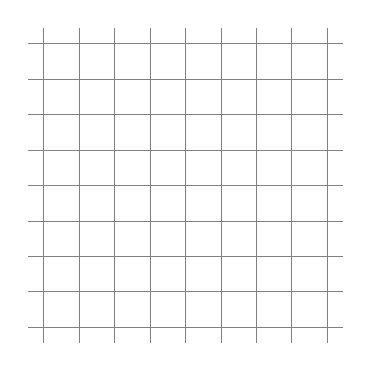
\begin{tikzpicture}
\draw[step=.45cm,gray,very thin] (-2,-2) grid (2,2);
\end{tikzpicture}\end{center}
\begin{center}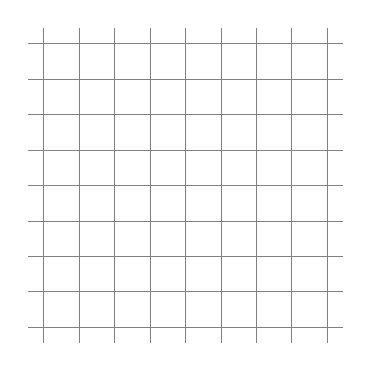
\begin{tikzpicture}
\draw[step=.45cm,gray,very thin] (-2,-2) grid (2,2);
\end{tikzpicture}\end{center}
\begin{center}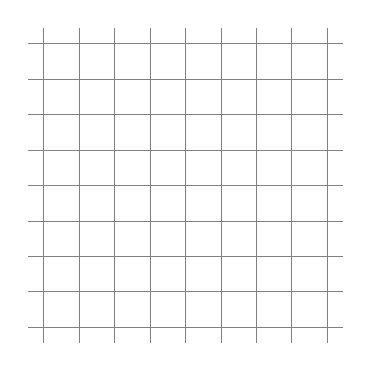
\begin{tikzpicture}
\draw[step=.45cm,gray,very thin] (-2,-2) grid (2,2);
\end{tikzpicture}\end{center}
\end{multicols}



\item Draw the lewis structure of the following compounds and indicate their polarities: \ce{CH4},  \ce{CH2Cl2},  \ce{CHCl3}.
\begin{multicols}{3}
 \begin{center}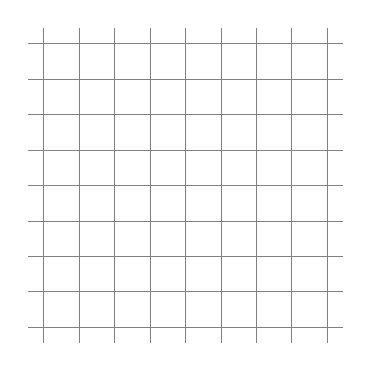
\begin{tikzpicture}
\draw[step=.45cm,gray,very thin] (-2,-2) grid (2,2);
\end{tikzpicture}\end{center}
\begin{center}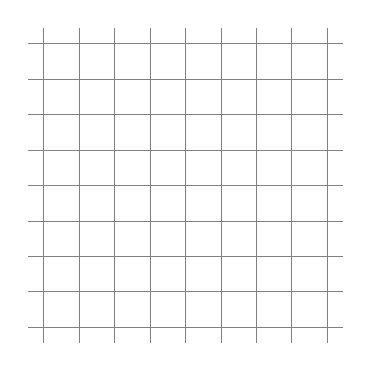
\begin{tikzpicture}
\draw[step=.45cm,gray,very thin] (-2,-2) grid (2,2);
\end{tikzpicture}\end{center}
\begin{center}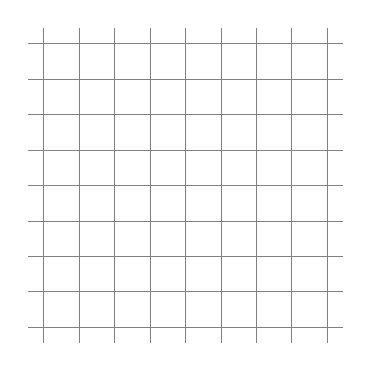
\begin{tikzpicture}
\draw[step=.45cm,gray,very thin] (-2,-2) grid (2,2);
\end{tikzpicture}\end{center}
\end{multicols}



  
\end{enumerate}
\end{fullwidth}




\newgeometry{right=5cm}
%\thispagestyle{sidebar}
\sidebar{%
  \vspace{1em}
  \vspace{1cm}
  \vfill
  \par\vspace*{1em}
}

\begin{landscape}\begin{centering}
\begin{tcolorbox}[tab2,tabularx={X|>{\hsize=5cm}Y|Y|Y|Y|Y|Y}]%%%% FANCY COLOR TABLE
\Large  Formula &
Lewis Structure\rot{\vspace{2.8cm}} &
\Large \# valence $e^-$ &
\Large \# $e^-$ pairs &
\Large Geometry &
\Large Angles &
\Large Polar?  \\\hline
 \Huge \ce{NH3}\rot{\hspace{3.8cm}}&   &   &   &  & &  \\\hline 
\Huge \ce{H2O}\rot{\hspace{3.8cm}} &   &   &   &  & &  \\\hline
 \Huge \ce{CH4}\rot{\hspace{3.8cm}}&   &   &   &  & & \\\hline 
 \Huge \ce{CH2Cl2}\rot{\hspace{3.8cm}} &   &   &   &  & &  \\\hline 
\end{tcolorbox}%%%% FANCY COLOR TABLE
\end{centering}
\end{landscape}

\begin{landscape}\begin{centering}
\begin{tcolorbox}[tab2,tabularx={X|>{\hsize=5cm}Y|Y|Y|Y|Y|Y}]%%%% FANCY COLOR TABLE
\Large  Formula &
Lewis Structure\rot{\vspace{2.8cm}} &
\Large \# valence $e^-$ &
\Large \# $e^-$ pairs &
\Large Geometry &
\Large Angles &
\Large Polar?  \\\hline
 \Huge \ce{CO2}\rot{\hspace{3.8cm}}&   &   &   &  & &  \\\hline 
\Huge \ce{CO3^{2-}}\rot{\hspace{3.8cm}} &   &   &   &  & &  \\\hline
 \Huge \ce{CH2O}\rot{\hspace{3.8cm}}&   &   &   &  & & \\\hline 
 \Huge \ce{SO2}\rot{\hspace{3.8cm}} &   &   &   &  & &  \\\hline 
\end{tcolorbox}%%%% FANCY COLOR TABLE
\end{centering}
\end{landscape}

\begin{landscape}\begin{centering}
\begin{tcolorbox}[tab2,tabularx={X|>{\hsize=5cm}Y|Y|Y|Y|Y|Y}]%%%% FANCY COLOR TABLE
\Large  Formula &
Lewis Structure\rot{\vspace{2.8cm}} &
\Large \# valence $e^-$ &
\Large \# $e^-$ pairs &
\Large Geometry &
\Large Angles &
\Large Polar?  \\\hline
 \Huge \ce{ICl4^-}\rot{\hspace{3.8cm}}&   &   &   &  & &  \\\hline 
\Huge \ce{OPCl3}\rot{\hspace{3.8cm}} &   &   &   &  & &  \\\hline
 \Huge \ce{PCl5}\rot{\hspace{3.8cm}}&   &   &   &  & & \\\hline 
 \Huge \ce{AlCl6^{3-}}\rot{\hspace{3.8cm}} &   &   &   &  & &  \\\hline 
\end{tcolorbox}%%%% FANCY COLOR TABLE
\end{centering}
\end{landscape}




\restoregeometry













\end{document}